\documentclass[11pt, letterpaper]{article}
\usepackage[utf8]{inputenc}
\usepackage[margin=1in]{geometry}
\usepackage{amsmath}
\usepackage{amssymb}
\usepackage{tikz}
\usepackage{float}
\usepackage{enumitem}
\usepackage{titlesec}

% Title Formatting
\titleformat{\section}{\large\bfseries}{\thesection}{1em}{}
\titleformat{\subsection}{\normalsize\bfseries}{\thesubsection}{1em}{}

% Meta Data
\title{\textbf{International Economics: Chapter 3 Problem Set}}
\author{Sean Balbale \\ Trinity College (Class of '27)}
\date{January 30, 2026}

\begin{document}

\maketitle

\section*{Problem 1}
\textbf{Restatement:} On one set of axes, sketch a fairly large production frontier concave from the origin.
(a) Starting near the midpoint on the production frontier, use arrows to show that the nation incurs increasing opportunity costs in producing more of X and more of Y.
(b) How does the slope of the production frontier change as the nation produces more of X? More of Y? What do these changes reflect?

\subsection*{Solution}

\begin{figure}[H]
  \centering
  \begin{tikzpicture}[scale=1.2]
    % Axes
    \draw[->, thick] (0,0) -- (6,0) node[right] {$X$};
    \draw[->, thick] (0,0) -- (0,6) node[above] {$Y$};

    % Production Possibility Frontier (Concave)
    \draw[thick, blue] (0,5) to[out=0, in=90] (5,0);
    \node[blue] at (5.2, 5.2) {PPF};

    % Midpoint A
    \filldraw (2.5, 3.53) circle (2pt) node[above right] {$A$};

    % Arrows showing movement and increasing cost
    % Moving toward X (down the curve)
    \draw[->, red, thick] (2.5, 3.53) -- (3.5, 2.5);
    \node[red, right, align=left] at (3.5, 2.5) {More $X$ \\ Higher Opp. Cost (lose more $Y$)};

    % Moving toward Y (up the curve)
    \draw[->, green!60!black, thick] (2.5, 3.53) -- (1.5, 4.3);
    \node[green!60!black, left, align=right] at (1.5, 4.3) {More $Y$ \\ Higher Opp. Cost (lose more $X$)};
  \end{tikzpicture}
  \caption{Concave Production Possibility Frontier showing Increasing Opportunity Costs.}
\end{figure}

\noindent \textbf{(b) Analysis:}
\begin{itemize}
  \item \textbf{Producing more X:} As the nation moves down the curve (producing more X), the slope of the production frontier (in absolute terms) increases/steepens. This indicates that the nation must give up increasingly larger amounts of Y for each additional unit of X.
  \item \textbf{Producing more Y:} As the nation moves up the curve (producing more Y), the slope decreases/flattens. This indicates that to produce each additional unit of Y, the nation must sacrifice increasingly larger amounts of X.
  \item \textbf{Reflection:} These changes reflect \textbf{increasing opportunity costs}. Resources are not perfectly homogeneous; some are better suited for X (e.g., flat land) and others for Y (e.g., hilly terrain). Shifting less suitable resources into an industry reduces efficiency and raises the opportunity cost.
\end{itemize}

\hrulefill

\section*{Problem 2}
\textbf{Restatement:} On another set of axes, sketch three community indifference curves, making the top two curves cross each other.
(a) Why have you drawn community indifference curves downward, or negatively, sloped?
(b) What does the slope of the curves measure? Why is the slope of each curve smaller for lower points?
(c) Which of the two intersecting indifference curves shows a greater level of satisfaction to the right of the point of intersection? To the left? Why is this inconsistent with the definition of indifference curves?

\subsection*{Solution}

\begin{figure}[H]
  \centering
  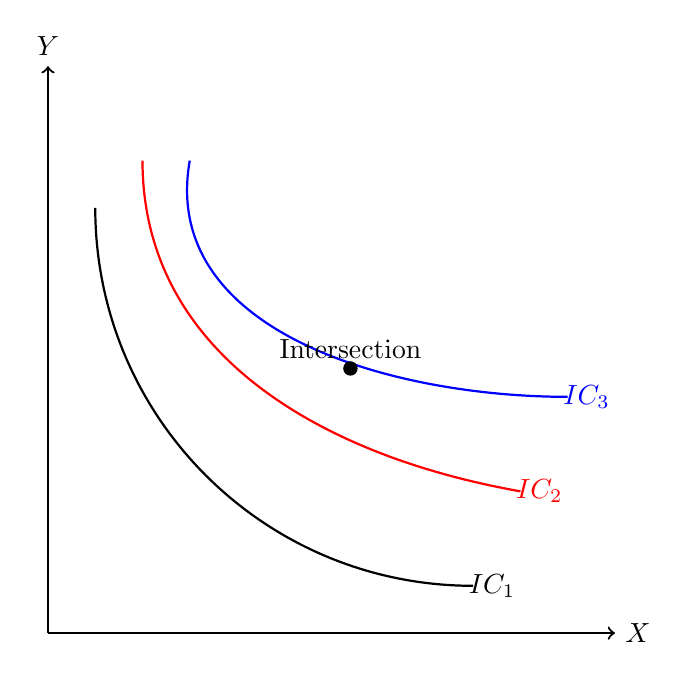
\begin{tikzpicture}[scale=1.2]
    % Axes
    \draw[->, thick] (0,0) -- (6,0) node[right] {$X$};
    \draw[->, thick] (0,0) -- (0,6) node[above] {$Y$};

    % Indifference Curve I (Standard)
    \draw[thick, black] (0.5, 4.5) to[out=270, in=180] (4.5, 0.5);
    \node at (4.7, 0.5) {$IC_1$};

    % Indifference Curve II (Intersecting)
    \draw[thick, red] (1, 5) to[out=270, in=170] (5, 1.5);
    \node[red] at (5.2, 1.5) {$IC_2$};

    % Indifference Curve III (Intersecting)
    \draw[thick, blue] (1.5, 5) to[out=260, in=180] (5.5, 2.5);
    \node[blue] at (5.7, 2.5) {$IC_3$};

    % Intersection Point
    \coordinate (Intersection) at (3.2, 2.8);
    \filldraw (Intersection) circle (2pt) node[above] {Intersection};
  \end{tikzpicture}
  \caption{Intersecting Community Indifference Curves (Logical Contradiction).}
\end{figure}

\noindent \textbf{(a) Negative Slope:}
The curves are negatively sloped because both X and Y are desirable economic goods. To maintain a constant level of utility, acquiring more X necessitates giving up some Y. A positive slope would imply the community has more of both goods yet remains at the same satisfaction level, violating the axiom of non-satiation.

\noindent \textbf{(b) Slope Measurement:}
The slope measures the \textbf{Marginal Rate of Substitution ($MRS_{xy}$)}—the amount of Y the nation is willing to forego to gain one unit of X while maintaining constant utility. The slope is smaller (flatter) at lower points due to \textbf{diminishing MRS}; as X becomes more abundant relative to Y, the nation values each additional unit of X less.

\noindent \textbf{(c) Intersection \& Inconsistency:}
To the right of the intersection, the higher curve ($IC_3$) offers greater satisfaction. To the left, the other curve ($IC_2$) is higher. This violates \textbf{transitivity}. If Point A is on $IC_2$, Point B is on $IC_3$, and they intersect at Point C, then $A=C$ and $B=C$, implying $A=B$. However, since A and B represent distinct baskets where one clearly dominates, this is a contradiction. Therefore, indifference curves cannot intersect.

\hrulefill

\section*{Problem 3}
\textbf{Restatement:} On one set of axes, sketch a community indifference curve tangent to the fairly flat section of a concave production frontier. On a second set, sketch a curve tangent to the steep portion of a different PPF.
(a) Draw the line showing the equilibrium-relative commodity price in isolation in each nation.
(b) Which is the commodity of comparative advantage for each nation?
(c) Under what condition would there be no comparative advantage?

\subsection*{Solution}

\begin{figure}[H]
  \centering
  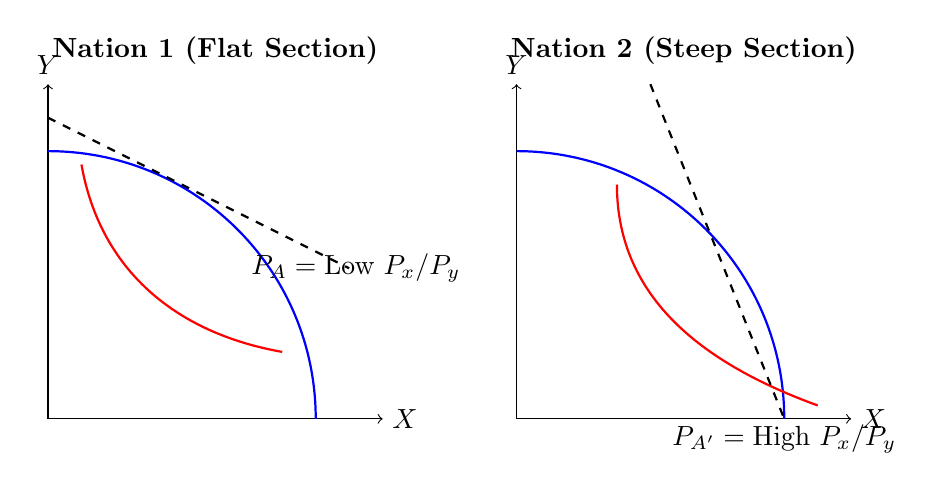
\begin{tikzpicture}[scale=0.85]
    % Nation 1
    \draw[->] (0,0) -- (5,0) node[right] {$X$};
    \draw[->] (0,0) -- (0,5) node[above] {$Y$};
    \node at (2.5, 5.5) {\textbf{Nation 1 (Flat Section)}};

    % PPF
    \draw[thick, blue] (0,4) to[out=0, in=90] (4,0);

    % Indifference Curve Tangent at Flat Section
    \draw[thick, red] (0.5, 3.8) to[out=280, in=170] (3.5, 1);

    % Price Line (Flat slope)
    \draw[dashed, thick] (0, 4.5) -- (4.5, 2.25);
    \node at (4.6, 2.25) {$P_A = \text{Low } P_x/P_y$};

    % Nation 2
    \begin{scope}[xshift=7cm]
      \draw[->] (0,0) -- (5,0) node[right] {$X$};
      \draw[->] (0,0) -- (0,5) node[above] {$Y$};
      \node at (2.5, 5.5) {\textbf{Nation 2 (Steep Section)}};

      % PPF
      \draw[thick, blue] (0,4) to[out=0, in=90] (4,0);

      % Indifference Curve Tangent at Steep Section
      \draw[thick, red] (1.5, 3.5) to[out=270, in=160] (4.5, 0.2);

      % Price Line (Steep slope)
      \draw[dashed, thick] (2, 5) -- (4, 0);
      \node at (4, -0.3) {$P_{A'} = \text{High } P_x/P_y$};
    \end{scope}
  \end{tikzpicture}
  \caption{Autarky Equilibria and Relative Prices.}
\end{figure}

\noindent \textbf{(b) Comparative Advantage:}
\begin{itemize}
  \item \textbf{Nation 1:} The price line is flatter, meaning a lower relative price of X ($P_x/P_y$). Nation 1 has a comparative advantage in \textbf{Commodity X}.
  \item \textbf{Nation 2:} The price line is steeper, meaning a higher relative price of X (and lower $P_y/P_x$). Nation 2 has a comparative advantage in \textbf{Commodity Y}.
\end{itemize}

\noindent \textbf{(c) No Comparative Advantage:}
This would occur if the autarky price lines in both nations had \textbf{identical slopes}, indicating identical relative commodity prices in isolation.

\hrulefill

\section*{Problem 4}
\textbf{Restatement:} (a) On the graphs of Problem 3, show the direction of specialization and the equilibrium point of production and consumption with trade. (b) How much does each nation gain compared to autarky?

\subsection*{Solution}

\begin{figure}[H]
  \centering
  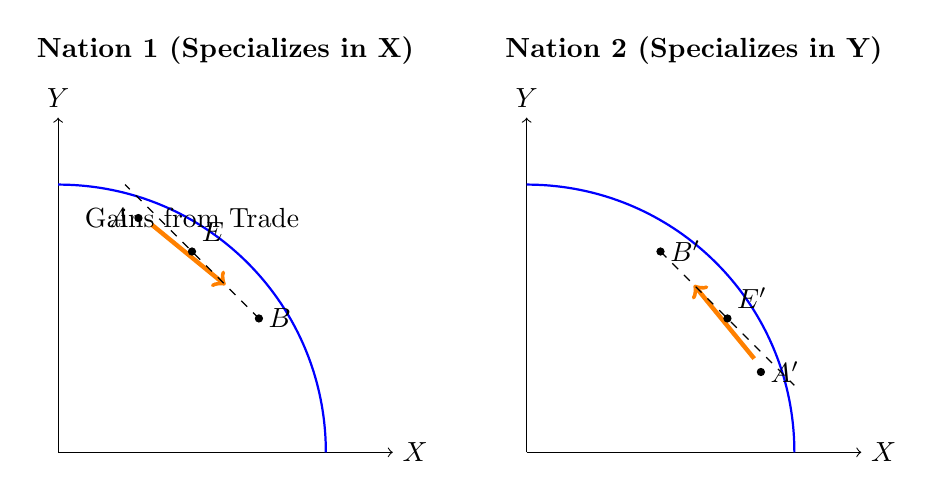
\begin{tikzpicture}[scale=0.85]
    % Nation 1
    \draw[->] (0,0) -- (5,0) node[right] {$X$};
    \draw[->] (0,0) -- (0,5) node[above] {$Y$};
    \node at (2.5, 6) {\textbf{Nation 1 (Specializes in X)}};

    % PPF
    \draw[thick, blue] (0,4) to[out=0, in=90] (4,0);

    % Autarky Point A
    \filldraw (1.2, 3.5) circle (1.5pt) node[left] {$A$};

    % Specialization Arrow
    \draw[->, ultra thick, orange] (1.4, 3.4) -- (2.5, 2.5);

    % Production Point B
    \filldraw (3, 2) circle (1.5pt) node[right] {$B$};

    % Trade Line
    \draw[dashed] (3, 2) -- (1, 4);

    % Consumption Point E
    \filldraw (2, 3) circle (1.5pt) node[above right] {$E$};
    \node at (2, 3.5) {Gains from Trade};

    % Nation 2
    \begin{scope}[xshift=7cm]
      \draw[->] (0,0) -- (5,0) node[right] {$X$};
      \draw[->] (0,0) -- (0,5) node[above] {$Y$};
      \node at (2.5, 6) {\textbf{Nation 2 (Specializes in Y)}};

      % PPF
      \draw[thick, blue] (0,4) to[out=0, in=90] (4,0);

      % Autarky Point A'
      \filldraw (3.5, 1.2) circle (1.5pt) node[right] {$A'$};

      % Specialization Arrow
      \draw[->, ultra thick, orange] (3.4, 1.4) -- (2.5, 2.5);

      % Production Point B'
      \filldraw (2, 3) circle (1.5pt) node[right] {$B'$};

      % Trade Line
      \draw[dashed] (2, 3) -- (4, 1);

      % Consumption Point E'
      \filldraw (3, 2) circle (1.5pt) node[above right] {$E'$};
    \end{scope}
  \end{tikzpicture}
  \caption{Production and Consumption Equilibria under Trade.}
\end{figure}

\noindent \textbf{(b) Analysis of Gains:}
Each nation gains the utility difference between the autarky point (tangency to a lower indifference curve) and the consumption point $E$ (on a higher indifference curve outside the PPF). While both nations gain, the distribution of gains depends on the terms of trade; the nation whose autarky price differs most from the world price captures the larger share of the gain.

\hrulefill

\section*{Problem 5}
\textbf{Restatement:}
(a) Determine the equilibrium-relative commodity price of the exports of commodity X with trade using the provided supply ($QS_x$) and demand ($QD_x$) schedules.
(b) What would happen if $P_x/P_y = 1\frac{1}{2}$?
(c) What would happen if $P_x/P_y = 1/2$?

\subsection*{Solution}

\begin{figure}[H]
  \centering
  \begin{tikzpicture}[scale=1.4]
    % Axes
    \draw[->, thick] (0,0) -- (7,0) node[right] {Qty of X ($Q_x$)};
    \draw[->, thick] (0,0) -- (0,4) node[above] {$P_x/P_y$};

    % Y-Axis Ticks
    \foreach \y/\label in {0.5/0.25, 1/0.5, 2/1, 3/1.5}
    \draw (0.1,\y) -- (-0.1,\y) node[left] {\label};

    % X-Axis Ticks
    \foreach \x/\label in {0/0, 2/40, 3/60, 3.5/70, 6/120}
    \draw (\x,0.1) -- (\x,-0.1) node[below] {\label};

    % Supply Curve (Nation 1)
    \draw[thick, blue] (0,0.5) -- (2,1) -- (3,2) -- (3.5,3);
    \node[blue, right] at (3.5,3) {$S_{exports}$};

    % Demand Curve (Nation 2)
    \draw[thick, red] (6,1) -- (3,2) -- (2,3);
    \node[red, right] at (2,3) {$D_{imports}$};

    % Equilibrium
    \filldraw (3,2) circle (2pt) node[above right] {$E$};
    \draw[dashed] (3,0) -- (3,2) -- (0,2);
  \end{tikzpicture}
  \caption{Partial Equilibrium Analysis of Trade.}
\end{figure}

\noindent \textbf{(a) Equilibrium Price:}
Equilibrium occurs where $QS_x = QD_x$. At $P_x/P_y = 1$, both quantity supplied and demanded equal 60. Thus, the equilibrium relative price is \textbf{1}.

\noindent \textbf{(b) At $P_x/P_y = 1.5$:}
$QS_x = 70$, $QD_x = 40$. There is a \textbf{surplus (excess supply)} of 30 units. This puts downward pressure on the price.

\noindent \textbf{(c) At $P_x/P_y = 0.5$:}
$QS_x = 40$, $QD_x = 120$. There is a \textbf{shortage (excess demand)} of 80 units. This puts upward pressure on the price.

\end{document}
